% This is "sig-alternate.tex" V2.1 April 2013
% This file should be compiled with V2.5 of "sig-alternate.cls" May 2012
%
% This example file demonstrates the use of the 'sig-alternate.cls'
% V2.5 LaTeX2e document class file. It is for those submitting
% articles to ACM Conference Proceedings WHO DO NOT WISH TO
% STRICTLY ADHERE TO THE SIGS (PUBS-BOARD-ENDORSED) STYLE.
% The 'sig-alternate.cls' file will produce a similar-looking,
% albeit, 'tighter' paper resulting in, invariably, fewer pages.
%
% ----------------------------------------------------------------------------------------------------------------
% This .tex file (and associated .cls V2.5) produces:
%       1) The Permission Statement
%       2) The Conference (location) Info information
%       3) The Copyright Line with ACM data
%       4) NO page numbers
%
% as against the acm_proc_article-sp.cls file which
% DOES NOT produce 1) thru' 3) above.
%
% Using 'sig-alternate.cls' you have control, however, from within
% the source .tex file, over both the CopyrightYear
% (defaulted to 200X) and the ACM Copyright Data
% (defaulted to X-XXXXX-XX-X/XX/XX).
% e.g.
% \CopyrightYear{2007} will cause 2007 to appear in the copyright line.
% \crdata{0-12345-67-8/90/12} will cause 0-12345-67-8/90/12 to appear in the copyright line.
%
% ---------------------------------------------------------------------------------------------------------------
% This .tex source is an example which *does* use
% the .bib file (from which the .bbl file % is produced).
% REMEMBER HOWEVER: After having produced the .bbl file,
% and prior to final submission, you *NEED* to 'insert'
% your .bbl file into your source .tex file so as to provide
% ONE 'self-contained' source file.
%
% ================= IF YOU HAVE QUESTIONS =======================
% Questions regarding the SIGS styles, SIGS policies and
% procedures, Conferences etc. should be sent to
% Adrienne Griscti (griscti@acm.org)
%
% Technical questions _only_ to
% Gerald Murray (murray@hq.acm.org)
% ===============================================================
%
% For tracking purposes - this is V2.0 - May 2012

\documentclass{sig-alternate-05-2015}
\usepackage[caption=false,font=footnotesize,labelfont=sf,textfont=sf]{subfig}
\usepackage{amsmath,amssymb}
\usepackage{multirow,booktabs,makecell}
\usepackage{color}
\graphicspath{{./pdf/}}

\begin{document}

% Copyright
\setcopyright{acmcopyright}
%\setcopyright{acmlicensed}
%\setcopyright{rightsretained}
%\setcopyright{usgov}
%\setcopyright{usgovmixed}
%\setcopyright{cagov}
%\setcopyright{cagovmixed}


% DOI
\doi{10.475/123_4}

% ISBN
\isbn{123-4567-24-567/08/06}

%Conference
\conferenceinfo{PLDI '13}{June 16--19, 2013, Seattle, WA, USA}

\acmPrice{\$15.00}

%
% --- Author Metadata here ---
\conferenceinfo{WOODSTOCK}{'97 El Paso, Texas USA}
%\CopyrightYear{2007} % Allows default copyright year (20XX) to be over-ridden - IF NEED BE.
%\crdata{0-12345-67-8/90/01}  % Allows default copyright data (0-89791-88-6/97/05) to be over-ridden - IF NEED BE.
% --- End of Author Metadata ---

\title{A Flexible Space-time Tradeoff on Hybrid Index with Bicriteria Optimization}
%\subtitle{
%[Extended Abstract]\titlenote{A full version of this paper is available as \textit{Author's Guide to Preparing ACM SIG Proceedings Using \LaTeX$2_\epsilon$\ and BibTeX} at \texttt{www.acm.org/eaddress.htm}}
%	}
%
% You need the command \numberofauthors to handle the 'placement
% and alignment' of the authors beneath the title.
%
% For aesthetic reasons, we recommend 'three authors at a time'
% i.e. three 'name/affiliation blocks' be placed beneath the title.
%
% NOTE: You are NOT restricted in how many 'rows' of
% "name/affiliations" may appear. We just ask that you restrict
% the number of 'columns' to three.
%
% Because of the available 'opening page real-estate'
% we ask you to refrain from putting more than six authors
% (two rows with three columns) beneath the article title.
% More than six makes the first-page appear very cluttered indeed.
%
% Use the \alignauthor commands to handle the names
% and affiliations for an 'aesthetic maximum' of six authors.
% Add names, affiliations, addresses for
% the seventh etc. author(s) as the argument for the
% \additionalauthors command.
% These 'additional authors' will be output/set for you
% without further effort on your part as the last section in
% the body of your article BEFORE References or any Appendices.

\numberofauthors{4} %  in this sample file, there are a *total*
% of EIGHT authors. SIX appear on the 'first-page' (for formatting
% reasons) and the remaining two appear in the \additionalauthors section.
%
\author{
% You can go ahead and credit any number of authors here,
% e.g. one 'row of three' or two rows (consisting of one row of three
% and a second row of one, two or three).
%
% The command \alignauthor (no curly braces needed) should
% precede each author name, affiliation/snail-mail address and
% e-mail address. Additionally, tag each line of
% affiliation/address with \affaddr, and tag the
% e-mail address with \email.
%
%AUTOR
%% 1st. author
\alignauthor Xingshen Song\\
\affaddr{College of Computer}\\
\affaddr{National University of Defense Technology}\\
\affaddr{Changsha, China}\\
\email{songxingshen@nudt.edu}
% 2nd. author
\alignauthor Yuexiang Yang\\
\affaddr{College of Computer}\\
\affaddr{National University of Defense Technology}\\
\affaddr{Changsha, China}\\
\email{yyx@nudt.edu}
% 3rd. author
\alignauthor Kun Jiang\\
\affaddr{School of Electronic and Information Engineering}\\
\affaddr{Xi'an Jiaotong University}\\
\affaddr{Xi'an, China}\\
\email{jk\_365@126.com}
\and  % use '\and' if you need 'another row' of author names
% 4th. author
\alignauthor Yu Jiang\\
\affaddr{College of Computer}\\
\affaddr{National University of Defense Technology}\\
\affaddr{Changsha, China}\\
\email{jiangyu@nudt.edu}
%AUTHOR
}
% There's nothing stopping you putting the seventh, eighth, etc.
% author on the opening page (as the 'third row') but we ask,
% for aesthetic reasons that you place these 'additional authors'
% in the \additional authors block, viz.
%\additionalauthors{Additional authors: John Smith (The Th{\o}rv{\"a}ld Group,
%email: {\texttt{jsmith@affiliation.org}}) and Julius P.~Kumquat
%(The Kumquat Consortium, email: {\texttt{jpkumquat@consortium.net}}).}
\date{12 July 2016}
% Just remember to make sure that the TOTAL number of authors
% is the number that will appear on the first page PLUS the
% number that will appear in the \additionalauthors section.

\maketitle
\begin{abstract}
Inverted Indexes are widely adopted in the vast majority of information systems.
Growing requirement for efficient query processing has motivated various compression techniques with different space-time characteristics.
While a single encoder yields a relatively stable point in the space-time tradeoff curve, flexibly transforming its characteristic along the curve to fit different IR tasks can be a better way to prepare the index.
Recent Research come out with an idea of combining different encoders within the same index, namely, exploiting access skewness by compressing frequently accessed regions with faster encoders and rarely accessed regions with succinct encoders.
Thus improving the efficiency while minimizing the compressed size.

However, these methods are either at a coarse granularity or algorithmically complex in practice.
To tackle these issue, we introduce the notion of \textit{Bicriteria Compression} to formalize the problem of optimally trading the compressed size and decompression time for inverted index.
We also adopt a Lagrangian relaxation algorithm to solve this problem by reducing it to a knapsack-type problem, which works in {\color{red}{$ O(n\log n) $}} time and $ O(n) $ space, with a negligible additive approximation.
We perform an extensive experiment to show that our method, which is faster and more theoretically complete, can optimally trading the space for bounded time, and vice versa.
\end{abstract}


%
% The code below should be generated by the tool at
% http://dl.acm.org/ccs.cfm
% Please copy and paste the code instead of the example below. 
%
\begin{CCSXML}
<ccs2012>
 <concept>
  <concept_id>10010520.10010553.10010562</concept_id>
  <concept_desc>Computer systems organization~Embedded systems</concept_desc>
  <concept_significance>500</concept_significance>
 </concept>
 <concept>
  <concept_id>10010520.10010575.10010755</concept_id>
  <concept_desc>Computer systems organization~Redundancy</concept_desc>
  <concept_significance>300</concept_significance>
 </concept>
 <concept>
  <concept_id>10010520.10010553.10010554</concept_id>
  <concept_desc>Computer systems organization~Robotics</concept_desc>
  <concept_significance>100</concept_significance>
 </concept>
 <concept>
  <concept_id>10003033.10003083.10003095</concept_id>
  <concept_desc>Networks~Network reliability</concept_desc>
  <concept_significance>100</concept_significance>
 </concept>
</ccs2012>  
\end{CCSXML}

\ccsdesc[500]{Computer systems organization~Embedded systems}
\ccsdesc[300]{Computer systems organization~Redundancy}
\ccsdesc{Computer systems organization~Robotics}
\ccsdesc[100]{Networks~Network reliability}


%
% End generated code
%

%
%  Use this command to print the description
%
\printccsdesc

% We no longer use \terms command
%\terms{Theory}

\keywords{Inverted Index; Bicriteria Compression; Lagrangian Relaxation}

\section{Introduction}\label{sec:intro}
Indexing is essential to efficiently manage growing data and perform quick queries in many information retrieval systems.
The use of inverted Indexes in web search engine is probably one of the most successful examples in IR.
Despite of the fact that it is a relatively old yet simple data structure, inverted index is extensible with supplementary information to answer different queries within much less space occupied.
Compression has been one of the most active field of inverted index research in the last decades, for it not only reduces the space occupancy, but also accelerates data transfer in I/O.
See \cite{catena2014inverted,trotman2014compression,zobel2006inverted} for a detailed survey.

Traditional inverted index is composed of two parts: \textit{dictionary} and \textit{posting lists}.
The former contains pointers mapping term to its corresponding posting list, while the latter contains the docid of the matching document, the frequency of occurrence in the document, and positional information (if to support phrasal and proximity matching).
The inverted index compression  we are talking about is usually concentrated in the compression of posting lists.

However, there exists a divergence between compressed size and decompression time,
since pursuing the minimization of size will undoubtedly impair decoding.
Encoders with different space-time treadoffs keep coming out to settle for requirements of various user scenarios \cite{lemire2015decoding,ottaviano2015optimal,ottaviano2014partitioned,petri2014score,silvestri2010vsencoding}.
Among these techniques, splitting posting list into \textit{blocks} (or \textit{chunks}) has been demonstrate to be an efficient way and widely adopted by many encoders.
For the reason that by keeping blocks separately accessible we can expect faster decoding speed and hierarchical structure.
In addition, variable-sized blocks can utilize the clustering property of list to beat the entropy \cite{moffat2000binary,silvestri2010vsencoding}.
Nonetheless, designers of information systems have to carefully choose one of these encoders to satisfy different IR tasks: whether to achieve optimal compression ratio/decoding speed, sacrificing the other one; or to balance them by adopting one proper encoder with finely tuned space-time tradeoff.

Since a single encoder has its own stable performance in the space-time tradeoff curve, it would be natural to ask for an encoder, which can trade the space occupancy and decoding time flexibly, to fit in different system requirement and device context.
An intuitive way to solve this problem is by combing different encoders into one index.
Namely, compressing the frequently accessed parts using a faster but less space-efficient encoder, and other parts using a slower encoder that gives better compression.

This idea is first adopted in \cite{yan2009inverted}.
However, the procedure of choosing encoders works at a posting list granularity, which is too coarse to obtain a flexible space-time tradeoff.
They also fail to explore complexity of the algorithm as it works on a empirical foundation.
Giuseppe et al. \cite{ottaviano2015optimal} explicitly define the Space-Constrained Expected Time Minimization problem: given a dataset $ D $ and an upper bound $ \cal S $ on its compressed size, the goal is to choose one proper encoder from an encoder set $ \cal E $ for each block of the index.
Thus minimizing the expected query processing time, provided that it can be compressed within $ \cal S $ space.
They then propose a linear time solution for this problem, which is quite straight forward.
Under two predefined dominance criteria, their algorithm works by enumerating all the advisable compression methods, then sorting them in an non increasing order by the time/space gain ratio of each advisable encoder on each block.
After this, a sequential scan and replace is able to find all the optional solutions for any possible budget constraint $ \cal S $.
Given the fact that each posting list is divided into fixed-sized blocks (say, 128 postings), whose total number is $ n $, and a set of $ k $ encoders, the algorithm finishes in $ \Theta(nk\log(nk)) $ time and $ O(nk) $ space.

By refining the granularity to block level and the carefully designed algorithm, they are able to find a solution with minimal query time.
Also, the approximation is additive, which is at most a block size larger than $ \cal S $.
However, the algorithm takes too much space to sort the compression options that it can be hardly fit into memory; second, since the sorting and sequential scan cannot be accelerated by parallel, the whole procedure is delay by them somehow; third, their solution is based on assumption that the posting lists are split into fixed-sized blocks, otherwise the compression options are hardly to sort and might take much more space. 

We argue that global ordering of the compression options for all the blocks is not a good idea, since it will lead to the above three shortcomings.
In this paper, we try to attack this problem from another perspective.
The main contributions are listed below:
\begin{enumerate}
	\item We introduce the conception of \textit{Bicriteria Compression} problem \cite{farruggia2014bicriteria} to extend the Space-Constrained Expected Time Minimization problem, which contains another dual problem.
	It changes the role of space/time by asking for the minimal compressed size, provided an upper bound $ T $ in its average query processing time or decompression time.
	By solving the \textit{Bicriteria Compression} problem  we can expect our compression method to be more universal for different scenarios.
	\item We reduce the problem into a Resource Constrained Shortest Path problem \cite{mehlhorn2000resource} over a weighted DAG $ \cal G $, however, edges in $ \cal G $ contain two penalties: space cost and time weight.
	Thus, the problem can be formalized using Lagrangian relaxation, we use the algorithm introduced in \cite{farruggia2014bicriteria} and \cite{handler1980dual} to settle in $ O(n\log n) $ time and $ O(n) $ space, while keeping the same additive approximation guarantee.
	\item Different from \cite{ottaviano2015optimal} which is a global search algorithm, our method amortizes the expect budget over each posting list.
	Thus, all the phrases of compression can be processed in a parallel way, runtime space requirement is also reduced without storing options in an index level.
	Our method is able to keep the additive approximation guarantee under different budgets, however, works much faster in practice.	
	{\color{red} Use data to demonstrate it}.
	\item we execute a preliminary set of experiments on two realistic dataset, GOV2 and Common Crawl, with AOL query log.
	Analysis shows that our method is able to obtain flexible tradeoffs under bicriteria compression.
	Its compressed size and query processing time is very competitive to the hybrid index in \cite{ottaviano2015optimal}, however, with more detailed description and more strict theoretic foundation.
\end{enumerate}

\section{Preliminaries}\label{sec: preliminaries}
\subsection{Index Structure and Compression}
Given a collection of \textit{D} documents, an inverted index can be seen as a big table mapping each unique \textit{term} to a\textit{ posting list} which contains all the document identifiers (called \textit{docid}) and the number of occurrences in the document (called \textit{frequency}), and possibly other information like the positions of each occurrence within the documents.
The set of terms is called \textit{lexicon}, which is relatively small compared to postings.
To rank the documents in response to a query, the posting list for the terms of the query must be traversed.
There is a vast variety of literature study on structures and query processing strategies, see \cite{ding2011faster,navarro2010dual} for a detailed survey.

Different orderings of the postings in the posting list change both the algorithm for ranked retrieval and the underlying representation of the postings in the inverted index.
Generally, there are two kinds of orderings, namely the docid-sorted and frequency-sorted, in docid-sorted index postings are sorted by docid in ascending order, allowing efficient compression and fast query processing; in frequency-sorted index postings are sorted by frequency in descending order and postings with same frequency are sorted by docid, an early termination can be reached for ranked query since the most promising postings are placed close to the start of the list.
A fatal problem with frequency-sorted index is that unordered docids are hard to compress, commercial search engines reportedly use the former obtain very good results by \cite{dimopoulos2013optimizing}.
The appropriate compression of docid-sorted index is the focus of our work.

To facilitate both compression and query processing, posting lists from the index are always considered separate data stream, components in each posting lists (docid, frequency and position) are stored in a non-interleaved way, and the lists of docid and position are usually sorted and transformed to the corresponding sequence of differences(or \textit{gaps}) between adjacent values.
Hence, the task of index compression is best viewed code sequences of integers of the form $x_{1},x_{2},x_{3},\ldots,x_{n}$ where $x_{i}\geqslant0$ for all $1\leqslant i\leqslant n$, and $n\geqslant1$ is the length of the sequence (\cite{anh2010index}).

Index compression is a relatively old and established topic in the literature of IR, researchers have summarized the previous work explicitly \cite{catena2014inverted,lemire2015decoding,silvestri2010vsencoding,trotman2014compression}.
The variety of compression techniques can be roughly divided into two classes, namely the \textit{integer-oriented encoders} and the \textit{list-oriented encoders}.

The integer-oriented encoders assign an unique codeword to each integer of the input list, then the compression procedure turns into a mapping or substitution from the integer space to code space.
As they compress integers without considering their neighborings, the integer-oriented encoders are also called oblivious encoders\cite{catena2014inverted}, such as \textit{unary code, Elias Gamma/Delta codes \emph{and} Golomb/Rice codes}.
Most integer-oriented encoders are hard to decode since they need bitwise operations to cross computer word boundaries, so byte/word-aligned encoders, are proposed to solve this problem, like \textit{Variable Byte} and \textit{Group Varint}, more importantly, they can be further improved by SIMD instructions of modern CPUs\cite{stepanov2011simd,trotman2014compression}.

List-oriented encoders are designed to exploit the cluster of neighboring integers, each time a fixed-sized or variable-sized group of integers is binary packed with an uniform bit width, providing equivalent compression ratio and faster decoding speed, the technique used by these encoders is called \textit{frame-of-reference}(FOR), or \textit{binary packing}\cite{goldstein1998compressing}.
Basically, their compression ratios are inferior to these of the first category as a batch of integers are encoded indiscriminately, and useless zeros are filled in the codeword to keep word-aligned.
However, when decoded, list-oriented encoders can obtain an entire block while the formers just decode one integer at a time.
More importantly, with the help of \textit{skip pointers} or \textit{skip list}, it is possible to step along the codewords compressed by list-oriented encoders and stop when the required number of blocks has been bypassed.
Some of these encoders are \textit{Simple Family}, AFOR and \textit{Patched} FOR (PFOR, OptPFOR and FastPFOR).

{\color{red}{we follow the settings used in \cite{ottaviano2015optimal}, that encoders in $ \cal E $ are chosen from list-oriented encoders and posting lists are uniformly split into fixed-size of 128.}}

{\color{red}{blocks are concatenated into one graph $ \cal G $.}}

\subsection{Pareto-optimal Compression}
Recently, researchers begin to use breakthroughs in succinct data structures to bear on the problems in inverted index compression.
Giuseppe et al. \cite{ottaviano2014partitioned} use pruned DAG \cite{ferragina2011optimally} to optimally partition posting list for minimal compression and convenient access.
Petri et al. \cite{petri2014score} describe an data structure combining pruned suffix tree and inverted index together to facilitate phrase-based ranking.
Our work is similar to these efforts, applying bicriteria compression to inverted index.

In our context, we are interested in optimally trading space occupancy with query processing time under specified space/time budget.
With respect to the notion of ``optimal", we introduce the concept of \textit{Pareto-Optimal Compression} to define it in a principled way: encoders achieve different points in the space-time trade-off curve, if to set the space occupancy and query processing time as two dimensions of the coordinate system.
Optimal ones are those extreme points whose performances are not worse than others in one dimension, and if to be optimized in any dimension, performances in the other two will get impaired accordingly.
Obviously there exists a set of Pareto-Optimal Compressions with different considerations.
As an extreme example, consider the two solutions: one is space-optimal compressed by Binary Interpolative Coding \cite{moffat2000binary} and the other one is time-optimal compressed by SIMD encoders.
That is, for any block of the posting list, we always choose to use either the space-efficient encoder or the time-efficient one.
However, in between these two extremes, we still have a plethora of encoders like PFOR and Simple-X.
Our goal is to move from one extreme to other by trading decompression speed for space occupancy, or vice versa.
Since there are $ k $ encoders for $ n $blocks, the key is to automatically and efficiently choose any of them for optimal tradeoffs.

\subsection{Directed Acyclic Graph}
By modeling index compression as an Directed Acyclic Graph $ \cal G $, finding the optimal solution can be reduced to the \textit{Single Source Shortest Path} problem over it.

$ \cal G $ is built as follows: a posting list can be treated as a list containing only positive integers $ L[0,m] $, where $ m $ is the number of postings.
Then each integer is represented by a vertex, plus a dummy vertex marking the end of the sequence.
$ \cal G $ is complete with $ O(m^2) $ edges, each edge is an exact correspondence of a partition in the $ L $.
The weight of an edge in the $ \cal G $ is equal to the cost in bits consumed by the partition.
The problem of fully partitioning $ L $ is converted to finding a path $\pi \in \Pi $ in $\mathcal{G}$, with its total edge weights $ \omega(\pi) $ minimized.

It has been commonly used in many list-oriented encoders \cite{song2016optimizing}.
These encoders usually partition a posting list into chunks of different lengths aligning to its local clusters.
Earlier ones like Fixed Binary \cite{anh2004index} and AFOR \cite{delbru2010adaptive} use a simple greedy search without backtracking.
Silvestri and Venturini introduce dynamic programming recurrence for VSEncoding \cite{silvestri2010vsencoding} while Guiseppe et al. resort to a more efficient approximation algorithm.

\begin{figure}
	\centering
	\subfloat[fixing $\varepsilon_{1}=0$, varying $\varepsilon_{2}$ from 0.1 to 1]{
		\label{fig:epsilon:b}
		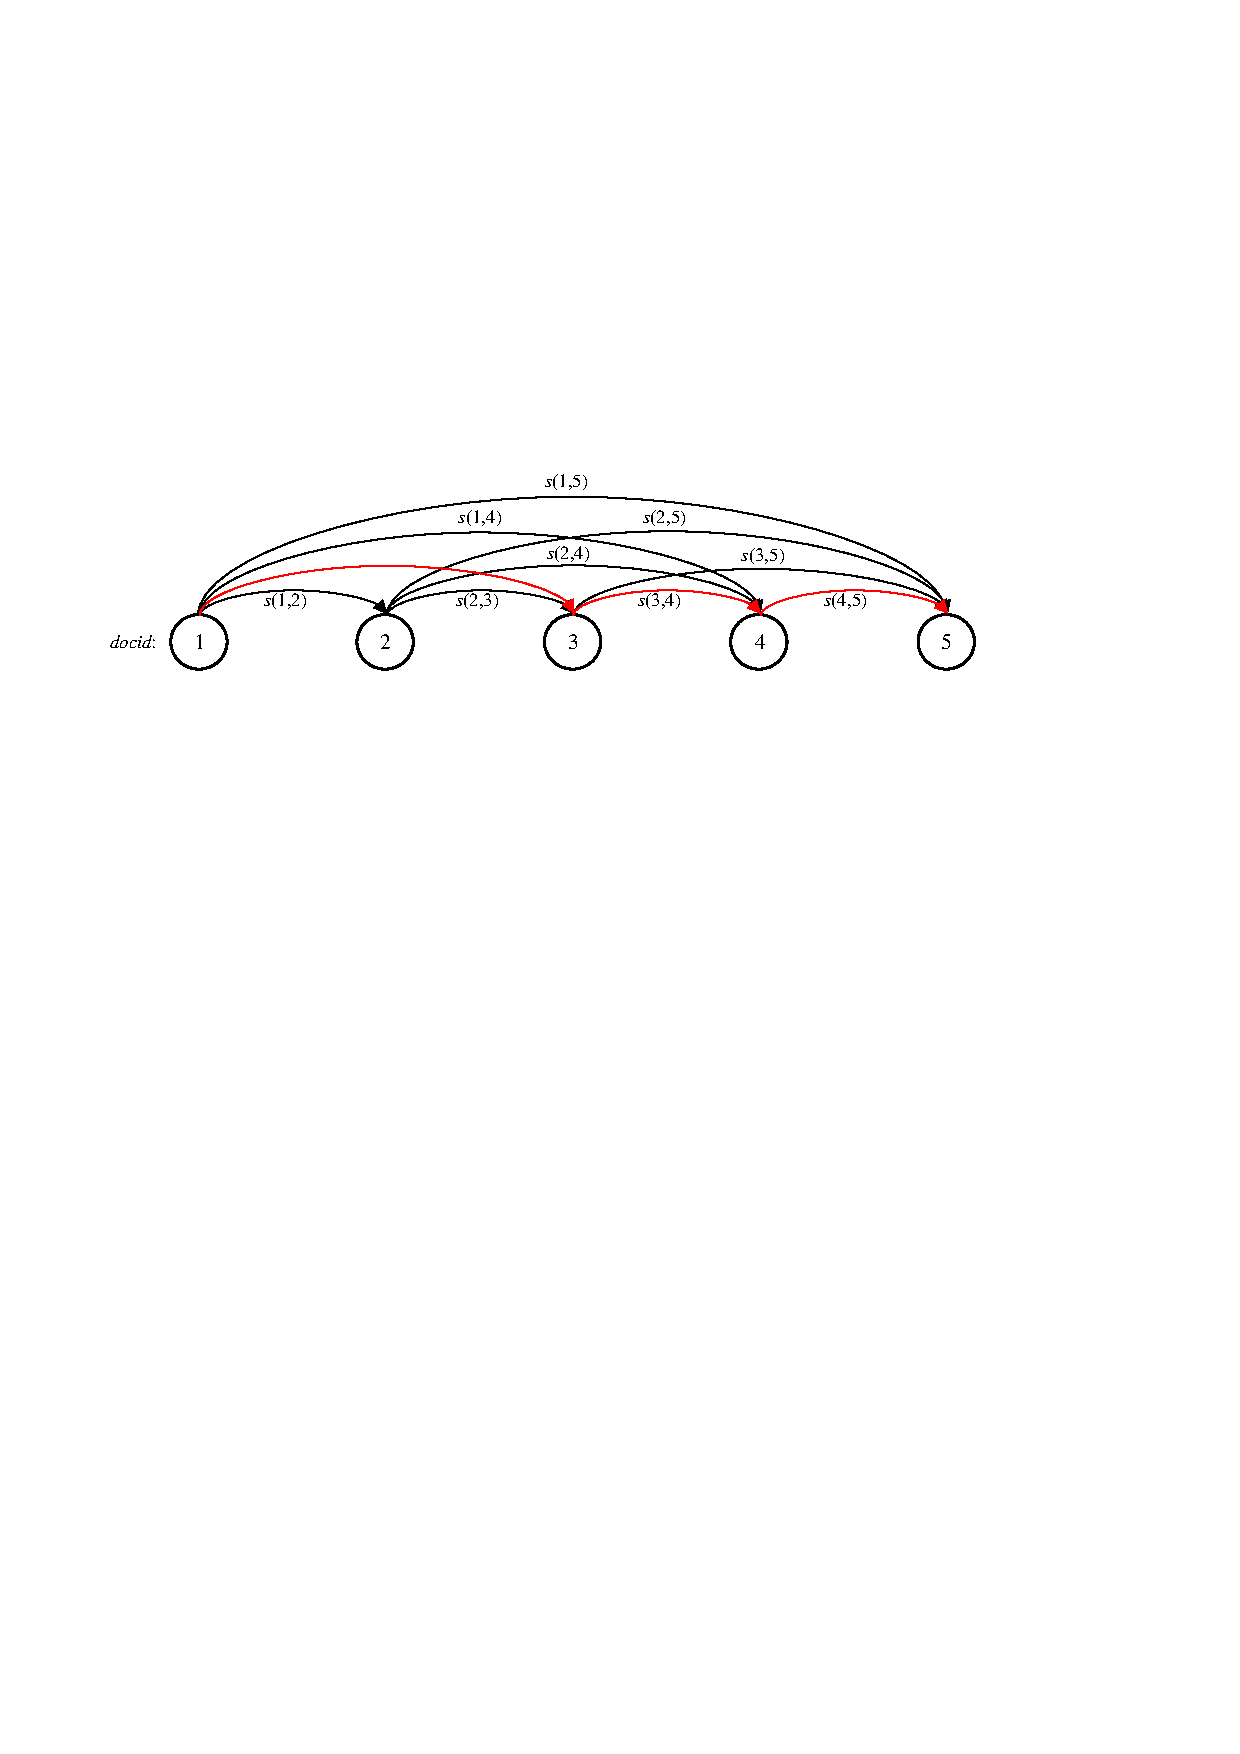
\includegraphics[width=1.0\linewidth]{sssp}
	}\\
	\subfloat[fixing $\varepsilon_{2}$ to values got above, varying $\varepsilon_{1}$ from 0 to 0.1]{
		\label{fig:phi:a}
		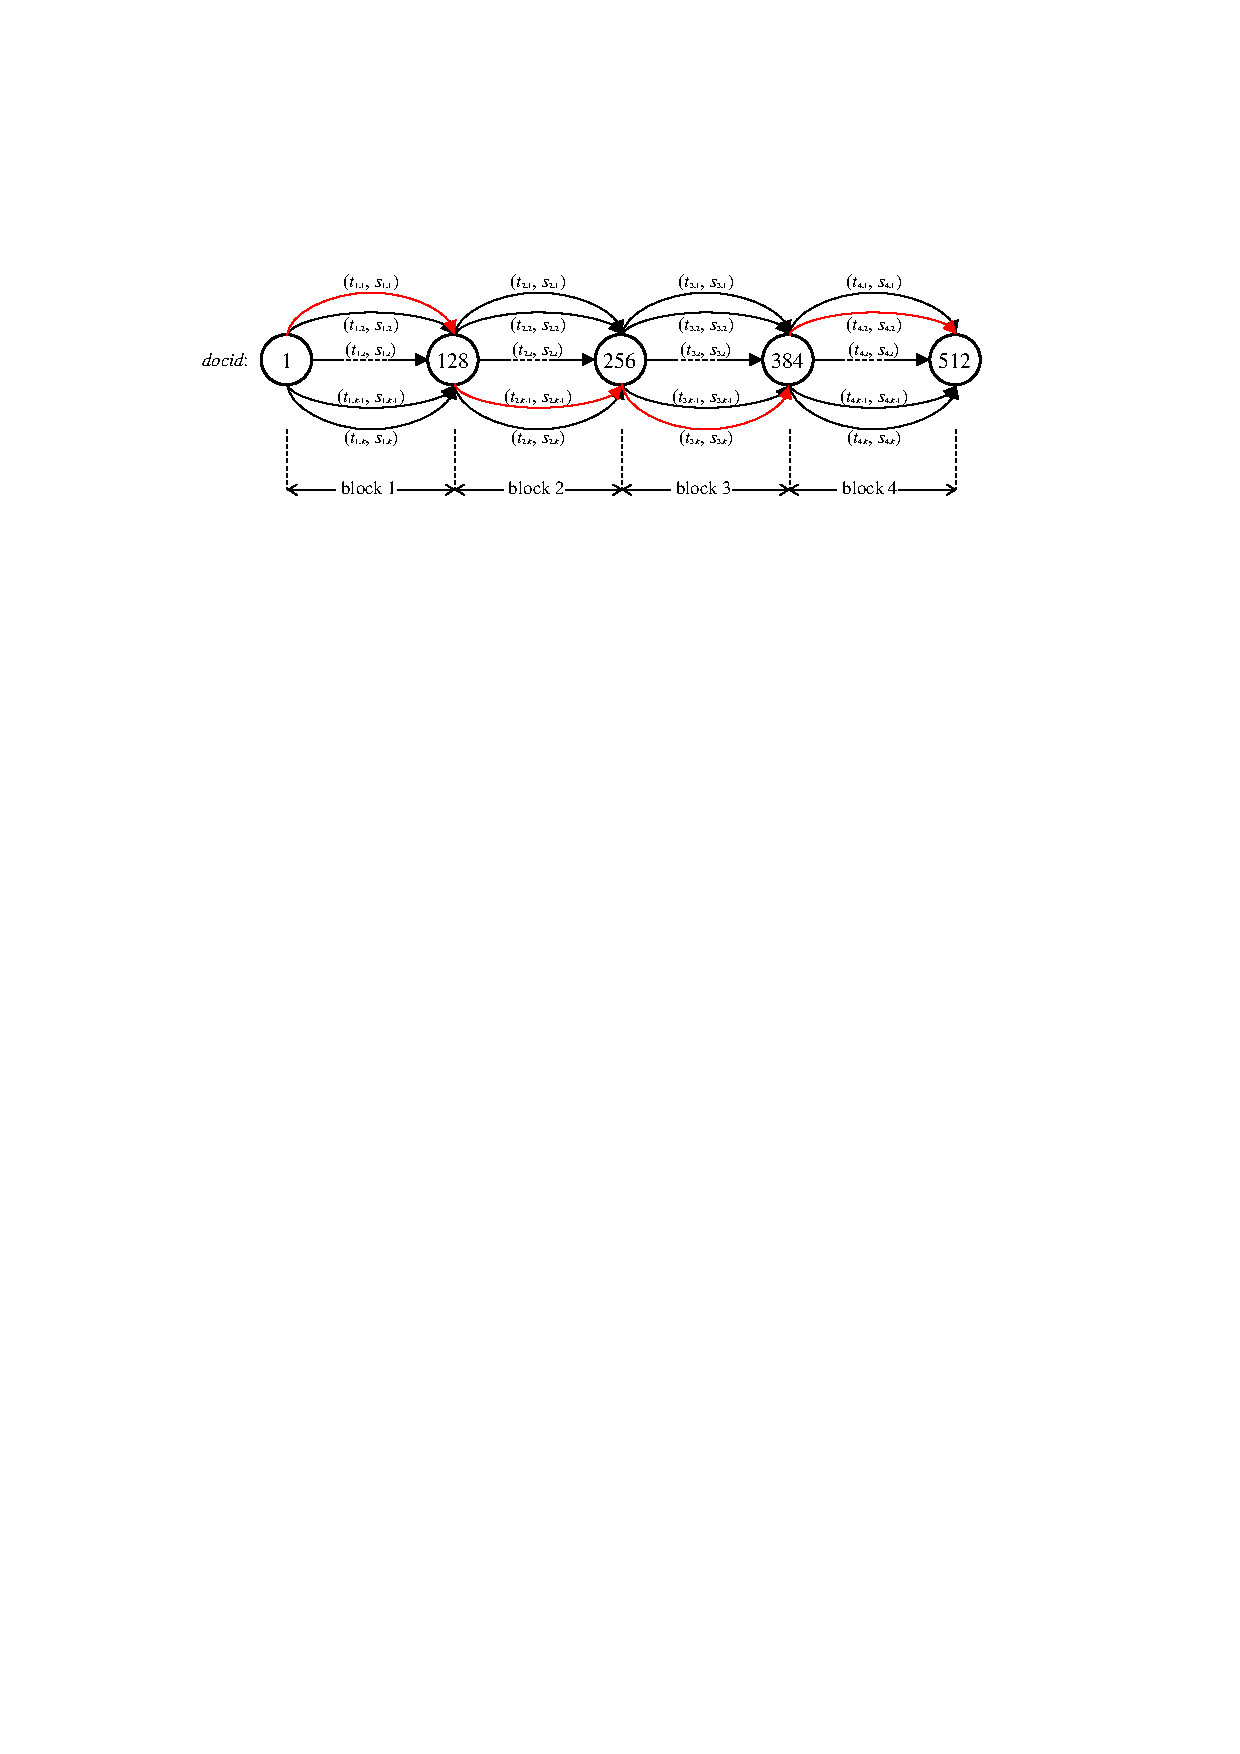
\includegraphics[width=1.0\linewidth]{rcsp}
	}
	
	\caption{Influences of the parameters $\varepsilon_{2}$ and $\varepsilon_{1}$ on two partitioning strategies.}
	\label{fig:parameter}
\end{figure}

However, our version of DAG $ \cal G $ has quite different definitions.
The above methods are designed to pursue space-optimal partitioning at all costs, without considering the decompression speed.
Our goal is to find one pareto-optimal solution under predefined space/time budget, in the new graph, each edge will have attached two weights: a \textit{time weight}, that accounts for the time to decompress a block, and a \textit{space cost}, that accounts for the number of bits needed to store a block associated to that edge.
The most notable contrast in our $ \cal G $ lies in the blocks of constant-size, which determine edge have fixed start and end points.
Between these points, there can be multiple edges to choose from due to the diversity of encoders.
So the total number of edges are exactly $ k \cdot \lceil \dfrac{m}{128} \rceil  $ rather than $ O(m^2) $.
For every path $ \pi $ from node 1 to node $ m $, we use $ s(\pi) = \sum_{i=1}^{l}\sum_{j=1}^{k}x_{i,j}s_{i,j} $ to represent the whole compressed size, where $ l= \lceil \dfrac{m}{128} \rceil$, $ x_{i,j} $ represents the choice of the encoder for block $ i $, and is 1 if the chosen encoder is $ j $ and 0 otherwise, $ s_{i,j} $ denotes the space cost of block $ i $ using encoder $ \mathcal{E}_j $.
Accordingly, the total decompression time is set to be $ t(\pi) = \sum_{i=1}^{l}\sum_{j=1}^{k}t_{i,j} $.
Thus we are able to rephrase the bicriteria compression problem into a Resource Constrained Shortest Path problem (RCSP) over the double weighted $ \cal G $, namely finding a path $ \pi $ whose decompression time $ s(\pi) < S $ while its compressed size $ t(\pi) $ minimized.
Symmetrically, we can also exchange the role of space/time resources, which asks minimal $ s(\pi) $ with $ t(\pi) < T $.
For the sake of convenience, we will consider the first formulation only in the rest of the paper. 

%The common foundation for the abovementioned methods is to recast the integer sequence $\mathcal{S} \left[ 0,n \right]$ to a particular DAG $\mathcal{G}$, each integer is represented by a vertex, plus a dummy vertex marking the end of the sequence.
%The graph $\mathcal{G}$ is complete, which means that for any $i$ and $j$ with $i < j \leqslant n$, there exists an edge connecting $v_{i}$ and $v_{j}$, denoted as $\left( v_{i}, v_{j} \right)$.
%In fact, the edge is an exact correspondence of a partition in the sequence $\mathcal{S}\left[i,j \right] $, the problem of fully partitioning $\mathcal{S}$ is converted to finding a path $\pi$ in $\mathcal{G}$, for instance, $\pi=\left( v_{0}, v_{i_{1}} \right) \left( v_{i_{1}}, v_{i_{2}} \right)\ldots\left( v_{i_{k-1}}, v_{n} \right)$ with $k$ edges corresponds to the partition $\mathcal{S}\left[0,i_{1}-1 \right]\mathcal{S}\left[i_{1},i_{2}-1 \right] \ldots\mathcal{S}\left[i_{k-1},n-1\right] $ of $k$ blocks.
%The weight of an edge in the graph is equal to the cost in bits consumed by the partition. Thus, the problem of optimally partitioning a sequence is reduced to the problem of Single-Source Shortest Path(SSSP) Labeling, as shown in Fig.~\ref{fig:sssp}.
%An intuitive way to solve this is to firstly set the cost of each vertex in $\mathcal{G}$ to $+\infty$, then an iteration starts from the left vertex to the rightmost, when it comes to a vertex $v_{j}$ with $0\leqslant j < n$, a subproblem of find the optimal path from $v_{j}$ to $v_{n}$ shows up, assuming the optimal path from $v_{0}$ to $v_{j}$ has been correctly computed.
%Each edge $\left( v_{j},v'\right)$ outgoing from $v_{j}$ will be assessed and cost of vertex $v'$ is updated if it becomes smaller. As can be seen, the time complexity of this algorithm is proportional to the number of edges in $\mathcal{G}$.

\section{Modeling the Problem}\label{sec: model}
%从这里想起来应该是把所有的posting list连接起来才对
In order to formulate the bicriteria compression problem, we need firstly model the space occupancy and decompression time of each block.
As stated in the Secion~\ref{sec: preliminaries}, we assume each posting list is split into blocks of fixed-size with a total number of $ n $, $ s_{i,j} $ is used to denote the compressed size of the \textit{i}th block encoded by the \textit{j}th encoder.
It can be obtained by compressing blocks using all the encoders before processing.
We follow \cite{ottaviano2015optimal} by setting $ T $ as the expected time to process queries from a given query set $ \cal Q $, and adopting the same model to predict the decompression time $ t_{i,j} $.
Then $ T $ is closely related to query processing strategy used and the distribution in $ \cal Q $.
We set $ t(\pi) = \sum_{i=1}^{n}x_{i,j}\hat{t}_{i,j} $, where $ \hat{t}_{i,j}=f_i t_{i,j} $, $ f_i $ is the number of times the \textit{i}th block was decoded while processing $ \cal Q $.
Also, $ f_i $ can be set to 1 if to measure the thorough decompression time of the index.

Now we can formulate our problem using Lagrangian relaxation into the famous RCSP as follows:
\begin{align}
 & \min_{\pi \in \Pi} t(\pi) \notag \\
 \text{s.t.}\quad & s(\pi) \leqslant \cal S \label{equ: RCSP}
\end{align}
By setting $ f(\pi) = t(\pi) $ and $ g(\pi) = s(\pi)- \mathcal{S} $, we may rewrite the Equation~\eqref{equ: RCSP} as
\begin{align*}
& \min_{\pi \in \Pi} f(\pi)  \\
\text{s.t.}\quad & g(\pi) \leqslant 0
\end{align*}

A brute-force solution to this problem would cost $ O(n^k) $ time and $ O(nk) $ space.
By adopting a dynamic programming approach proposed in \cite{lawler2001combinatorial}, both time and space can be reduced to $ \Theta(n\mathcal{S}) $, which is $ O(m^{2}\log m) $ at its worst.
Unfortunately this bound is still unacceptable is practice.

To efficiently solve the problem we introduce the Lagrangian function to relax the constraint $ g(\pi) \leqslant 0 $:
\begin{align}
L(\mu,\pi) = f(\pi)+\mu g(\pi) \label{equ: L(u,pi)} \\ 
\intertext{and let}
L(\mu) = \min_{\pi \in \Pi} L(\mu,\pi) \label{equ: L(u)}
\end{align}
\noindent $ \mu $ is the Lagrangian multiplier following $ \mu \geqslant 0 $.
It has been shown that this problem can be solved in linear time by solving this dual problem \cite{handler1980dual}.
Let $ \pi $ be the path we find, and $ \pi^\star $ be the optimal path of the RCSP problem.
At the end of Section~\ref{sec: our alg}, we will have proved the following theorem:
\newtheorem{theorem}{Theorem}
\begin{theorem}
	$ \pi $ can be computed in $ O(\log n) $ time and $ O(n) $ time with its time cost $ t(\pi) \leqslant f(\pi^\star) + t_{max} $ and space cost $ s(\pi) \leqslant S + 2s_{max} $.
\end{theorem}
Here we use $ s_{max} $ and $ t_{max} $ to denote the maximum space/time cost of one block.

\section{Our approximation Algorithm}\label{sec: our alg}
In this section we turn to the algorithm which solves the Lagrangian relaxation problem.
Recall the algorithm in \cite{ottaviano2015optimal}, which first sorts all the possible encodings of each block across the whole index, then adopts a greedy search to scan the sorted list and replace a space-optimal solution with faster encodings until the space budget $ S $ is reached, thus meeting with its additive guarantee.

Our algorithm works in a quite different way, its procedure can also be divided into two phase.
In the first phase, we adopt the cutting-plane algorithm to solve the Lagrangian dual problem introduced in \cite{handler1980dual}.
This algorithm starts from two extreme paths (say, $ \pi(0) $ and $ \pi(\infty) $) and fuses them to get a new path $ \pi' $, then recursively fuses $ \pi' $ with one of the former path until
a lower bound of $ L(\mu,\pi) $ is reached.
Thus we get an instantiation of $ \mu^\star $ corresponding to the maximal value of $ L(\mu) $, and a pair of paths $ (\pi_l,\pi_r) $ which are optimal for $ L(\mu^\star) $ and such that $ g(\pi_l) \geqslant 0 $ and $ g(\pi_r) \leqslant 0 $.

In case one of the two path has its space cost $ s(\pi_r) = S $, then its time cost is the optimal one of $ t(\pi^\star) $.
Unfortunately, this rarely occurs in practice and in most cases we have to tackle duality gap between $ \pi_l $ and $ \pi_r $.
In the second phase, we will execute a sequential exchange of edges from both paths.
After that, we will be able to get an optimal path whose time and space costs better approximate the budget.

\subsection{Solving the Dual Problem}
This phase mainly contributes to the fusion of two extreme paths, one of which is space-optimal while the other one is time-optimal, thus making the fused path converges gradually to the given range through an finite iteration.
The key step stays in generating the optimal path $ \pi' $ for $ \mu $ in each iteration.

Notice that in Equation~\eqref{equ: L(u,pi)} we have $ \mu \geqslant 0 $ and $ g(\pi) \leqslant 0 $, thus $ L(\mu,\pi) $ representing $ f(\pi) $ adding a negative number.
As we are trying to find a minimal $ f(\pi) $, we get the following equation:
\begin{equation}
L(\mu) \leqslant f(\pi^\star) \label{equ: maximum}
\end{equation}
\noindent For every $ \mu \geqslant 0 $.
Therefore, an best lower bound for the optimal path in RCSP can be found by solving its dual problem defined as 
\begin{equation}
L^\star = L(\mu^\star) = \max_{\mu \geqslant 0} L(\mu) =\max_{\mu \geqslant 0} \min_{\pi \in \Pi} \left[ f(\pi) + \mu g(\pi) \right]
\end{equation}

Now the problem has been converted from searching for an optimal path to a linear programming calculating maximal $ L(\mu) $, where each path defines a feasible region.
And our goal is find out the vertex which maximize $ L(\mu) $ from the convex hull defined by the intersection of paths.

However, it is impossible to figure out the convex hull using traditional simplex method since there can be $ O(n^k) $ paths.
Actually we only need a small part of them to heuristically pruning out unfeasible paths and determining the maximal $ L(\mu) $.
\begin{figure}
	\centering
	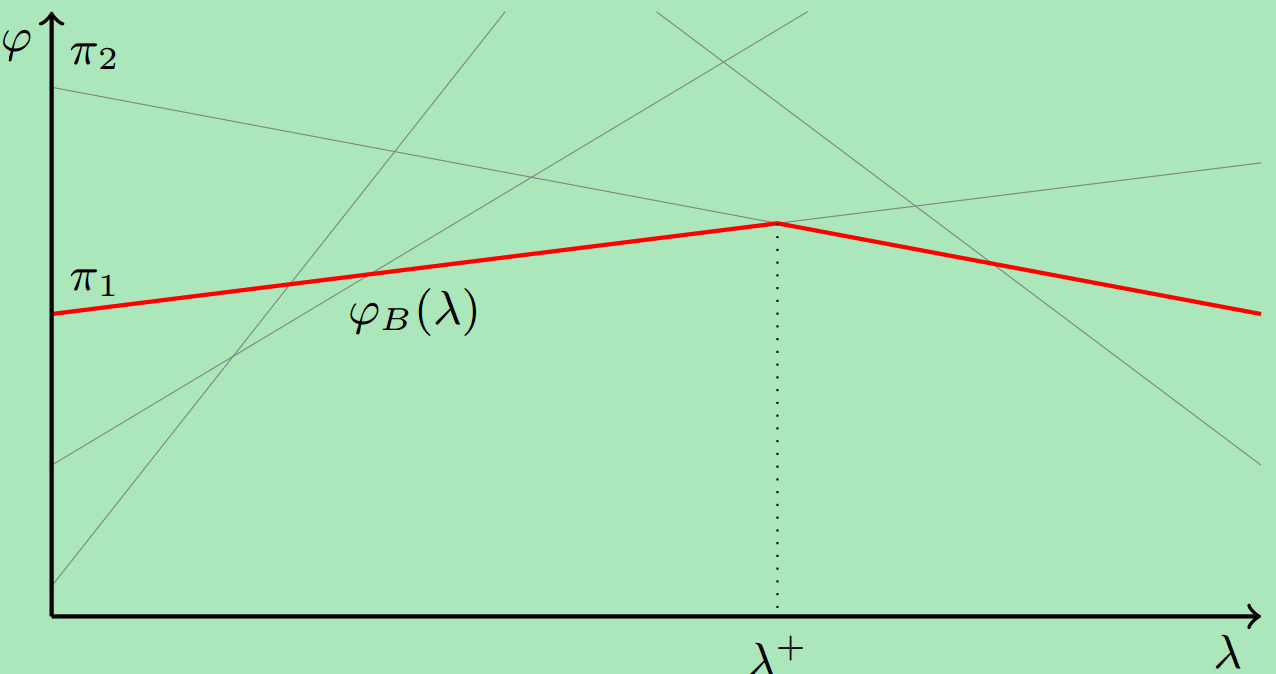
\includegraphics[width=0.9\linewidth]{intersection}
	\caption[sssp]{Here is a DAG for sequence with 6 integers represented using gap(differences between them).
	{\color{red}{the horizontal line of LB and UB}}	}
	\label{fig: intersection}
\end{figure}

The procedure can be best explained geometrically.
Each path in $ \Pi $ may be associated in $ (\mu, L)($ space with a line of the form $ L = f(\pi) + \mu g(\pi) $, where $ f(\pi) $ is the intercept along the L-axis and $ g(\pi) $ is the slope of the line.
Feasible paths have a non-positive slope (sice $ g(\pi) \leqslant 0 $) and feasible paths have a positive slope.
As mentioned above, we only keep a pair of paths in hand and recursively intersect them to determine the point $ (\mu',L') $.
Note $ L(\mu) $ represents the lower envelope of the all the paths generated so far, so it will consist of two lower segments of the corresponding paths and the point of intersection will maximize $ L(\mu) $.
If there exists another path $ L(\mu') $ ( generated using $ \mu' $) which further tightens the lower envelope $ L' $, then we can have the maximum value of $ L(\mu) $ more close to $ L^\star $ from above.
So the whole procedure works to find a minimal maximum of $ L(\mu) $ since $ L(\mu') \geqslant L(\mu^\star) $.
The iteration stops once $ L(\mu') $ cannot be reduced or we find a path $ \pi^\circ \in \Pi $ with $ g(\pi) = 0 $ and $ L(\mu') = L(\mu', \pi^\circ) < L' $, then the point $ (\mu', L(\mu')) $ represents the optimal solution for the dual problem.

For a given $ \mu $, a path is called $ \mu $-\textit{optimal} if its Lagrangian cost $ L(\pi,\mu) $ equals to the value of $ L(\mu) $ in equation~\eqref{equ: L(u)}.
Consider the initial step, which is to find two extreme paths with respect to function $ f(\pi) $ and $ g(\pi) $ respectively.
Since $ \mu \in [0,+\infty) $ and for each path $ L(\mu) $ represents a monotonic line in $ (\mu,L) $ space.
Naturally, the extreme path exists at $ \mu = 0 $ and $ \mu=\infty $.
Let $ \pi(\mu) $ denote an $ \mu $-\textit{optimal} path associating with $ \mu $,
$ \pi(0) $ corresponds to $ L(0) = \min\{f(\pi)|\pi \in \Pi\} $ which is the minimum of $ f(\pi) $, if $ g(\pi) \leqslant 0 $ then $ \pi(0) $ is also optimal for RCSP.
And $ \pi(\infty) $ corresponds to the minimum of $ g(\pi) $, if $ g(\pi(\infty)) > 0 $, then there will be no solution for RCSP.

It is easy to prove that $ \pi(0) $ and $ \pi(\infty) $ are exactly time-optimal and space-optimal paths in our scenario.
We start by setting $ (\pi(0),\pi(\infty)) $ as $ (\pi_l,\pi_r) $, each time we intersect them, we get the point $ \mu' = (f_l - f_r)/(g_r-g_l) $ and $ L'= f_l + \mu' g_l $.
Then a new path $ \pi' $ is generated as $ L(\mu') $, if $ g(\pi') < 0 $, $ \pi_r $ will replaced by $ \pi' $ and vice versa.
The procedure terminates when $ L(u') = L' $ or $ g(\pi') = 0 $.
It has been shown the number of iterations is $ O(\log(n $$ s_{costs} $$ t_{costs})) $ \cite{mehlhorn2000resource}, where $ s_{costs} $ and $ t_{costs} $ represent the block space/time cost in integers, in our scenario these two are negligible constant since block size is fixed to 128.

It remains to describe how to generate an $ \mu $-\textit{optimal} path $ \pi' $ given the point of intersection $ (\mu',L') $.
A brute force search along the whole graph for $ \pi' $ by evaluating its Lagrangian cost is impossible,
even our version of  $ \cal G $ has already reduced its number of edges from $ O(n^2) $ to $ O(nk) $ by fixing the edge length.
However, fixing the size of blocks indeed bring one significant advantage that blocks are kept isolated from each other.
Thus we can break this problem into numerous subproblems of selecting proper encodings for each block, which minimize its Lagrangian cost given any $ \mu \geqslant 0 $.
Finally we can sum their space/time costs together without collision.
Namely,
\begin{equation*}
L(\mu,\pi) = L(\sum_{i=1}^{n} e_i, \mu)=\sum_{i=1}^{n}L(e_i,\mu)
\end{equation*}
Here $ e_i $ denotes edges in path $ \pi $.

To find the appropriate encodings we need first recall the dominance criteria proposed in \cite{ottaviano2015optimal}: a) Let \textit{p} and \textit{q} be two items in the same class \textit{i}.
Item \textit{q} is dominated by item \textit{p} if $ s_{i,p} \leqslant s_{i,q} $ and $ \hat{t}_{i,p} < \hat{t}_{i,q} $;
b) Let \textit{p}, \textit{q} and \textit{r} be three items in the same class such that $ s_{i,p} < s_{i,q} < s_{i,r} $ and $ \hat{t}_{i,p} \geqslant \hat{t}_{i,q} \geqslant \hat{t}_{i,r} $.
Item \textit{q} is dominated by \textit{p} and \textit{r} if the following condition holds $ \frac{\hat{t}_{i,p} - \hat{t}_{i,q}}{s_{i,p} - s_{i,q}} \geqslant \frac{\hat{t}_{i,q} - \hat{t}_{i,r}}{s_{i,q} - s_{i,r}} $.
After applying these criteria, for each block we have the dominated items pruned from $ \cal G $ and the rest items sorted in ascending order by their space cost.
Also a time/space gain ratio between adjacent items is define as $ \lambda_{i,j} = \frac{\hat{t}_{i,j} - \hat{t}_{i,j-1}}{s_{i,j-1} - s_{i,j}} $.

Let $ L_{i,j} $ denote the Lagrangian cost of the \textit{i}th block encoded by the \textit{j}th encoder.
Our key observation is that the minimal Lagrangian cost of each block can be found by finding the smallest $ \lambda_{i,j} $ that approximates $ \mu $ from above.
As shown in the following equation:
\begin{equation}
\begin{split}
L_{i,j} - L_{i,j-1} &= f(e_{i,j}) - f(e_{i,j-1}) + \mu (g(e_{i,j}) - g(e_{i,j-1})) \\
	&= \hat{t}_{i,j} - \hat{t}_{i,j-1} + \mu (s_{i,j} - s_{i,j-1}) \\
	&= \lambda_{i,j}(s_{i,j-1} - s_{i,j}) + \mu (s_{i,j} - s_{i,j-1}) \\
	&= (s_{i,j} - s_{i,j-1})(\mu - \lambda_{i,j})
\end{split}
\end{equation}
Since $ s_{i,j} > s_{i,j-1} $, encodings with $ \lambda_{i,j} \geqslant \mu $ will reduce the cost of current block,
and the minimal $ L_i $ is exactly $\min\{ \lambda_{i,j}| \lambda_{i,j} \geqslant \mu \}  $.

The set of $ \lambda $s is sorted once and accessed many times, this can be done in constant time with simple operations since there are only $ k $ encoders to choose.
Here, we emphasize that the above operations are carried out within a block level rather than the whole index.
To generate a 1-\textit{n} path would obviously cost $ O(nk) $ time and space.
Recall the number of iterations previously mentioned, the dual problem can be solved in $ O(\tilde{n} $$ \log(n$$ s_{costs} $$ t_{costs})) $ time and $ O(\tilde{n}) $ space, where $ \tilde{n} = nk $ is the $ \cal G $'s size.

\subsection{Closing the Gap}
Upon termination of the iteration we have two paths $ (\pi_l,\pi_r) $ which specify a lower bound and an upper bound of the minimal value $ f(\pi^\star) $.
From Equation~\eqref{equ: maximum}, we know the lower bound is the intersection point, namely $ LB =  L(\mu^\star) $; also, any path $ \pi $ with $ g(\pi) \leqslant 0 $ generated during the iteration is a feasible solution for RCSP, and the best value for upper bound is $ f(\pi_r) $ from the last path $ \pi_r $.
Thus we have the bound $ L(\mu^\star) \leqslant f(\pi^\star) \leqslant f(\pi_r) $, which is also shown in Figure~\ref{fig: intersection}.

Obviously, if $ L(\mu^\star) = f(\pi_r) $ or any one path in $ (\pi_l,\pi_r) $ satisfies $ g(\pi) = 0 $, there would be no duality gap between solutions to RCSP and its dual problem.
However, this rarely happens in practice.
Therefore we have to deal with duality gap until an optimal path is found for RCSP.

Following \cite{farruggia2014bicriteria}, we reuse the path-swapping algorithm introduced for this task.
The notion of \textit{path swapping} can be explained as follow: given a pair of paths $ (\pi_l,\pi_r) $, we first choose one point $ v $ along the paths arbitrarily as a \textit{pivot}, then we create two new paths $ (\pi_1,\pi_2) $ by exchanging edges before the pivot of $ (\pi_l,\pi_r) $.
In our context, the algorithm is greatly simplified since edges of all paths have fixed start and end points, we do not need to consider cases where edges are split or merged for shared pivot.
It has been shown that any path generated by path-swap is off at most off at most $ t_{max} $ in time and $ s_{max} $ in space from being a $ \mu $-optimal path, $ t_{max} $ and $ s_{max} $ denote maximum time/space cost of one block.
Indeed, the operation is executed on two closely resembled $ \mu $-optimal paths edge-wise.
By moving the pivot from left to right, we are actually substituting path $ \pi_l $ for path $ \pi_r $ edge by edge.
These intermediate paths are naturally bounded by $ \pi_l $ and $ \pi_r $, and there definitely exists a $ \mu $-optimal path whose cost is at most one block-size smaller than these paths.

The block-wise operation also guarantees paths generated using two adjacent pivots differ from each other by at most $ t_{max} $ and $ s_{max} $.
A left-to-right scanning is sufficient to change the Lagrangian cost from $ L(\mu^\star) $ to $ f(\pi_r) $ in a appropriate granularity, and find an optimal solution for $ f(\pi^\star) $ with an additive approximation.
During the procedure, we only need an accumulator to store the current pivot and time/space cost, thus the path-swap algorithm can be done in $ O(n) $ time and $ O(1) $ space.

\section{Experiments}\label{sec: experiments}
In order to provide an experimental evaluation of the proposed compression technique, we have implemented our algorithm in C++.
All the code related with experiments is available at GitHub\footnote{Anonymized for review}.
In special, we would like to compare its efficiency and compression effectiveness with the original method in \cite{ottaviano2015optimal}, so we retain most configurations of their experiments to avoid interference from other factors.

\subsection{Experimental Setup}
We choose the same encoder set $ \cal E $ used in \cite{ottaviano2015optimal}, namely Interpolative, PFD(\textit{h}) and Varint-G8IU.
Here \textit{h} stands for exception bit length, and different \textit{h} are treated as different encoders.
Blocks with less than 128 postings are always compressed by Interpolative.

We use the posting lists extracted from the following two collections: \textbf{TREC GOV2} and \textbf{Common Crawl}.
TREC GOV2 is a crawl of the \textbf{.gov} sites used in TREC 2004 Terabyte Track, which consists of 25.2 million documents and 15.3 million terms.
Common Crawl is a corpus of web crawl data composed of over 5 billion web pages over last 7 years, and it keeps growing until now.
The crawl data is stored using WARC 1.0 format with about 541 TB in size.
This whole collection is freely available on Amazon S3\footnote{\url{http://commoncrawl.org/}}. 


Since the Common Crawl corpus is too large to fit in one machine, we only extract a small part of the data crawled in February 2016.
Documents from these two collections are prepared by applying Porter stemmer after removing stopwords, then the docids are reordered by the lexicographic order of URLs.
Table~\ref{tab: collection statistics} compares these two collections using some basic statistics.

\begin{table}
	\centering
	\caption{Collection statistics for GOV2 and Common Crawl}
	\renewcommand{\arraystretch}{1.0}
	\begin{tabular}{l*{2}{r}}
		\toprule
		& \multicolumn{1}{c}{GOV2} & \multicolumn{1}{c}{Common Crawl} \\
		\midrule
		Documents & 25,203,921 & 17,157,948 \\
		Terms  & 15,324,160 & 51,990,893 \\
		Pointers & 4,655,778,182 & 9,118,361,737 \\
		Document Length(avg.) & 645.25 & 2151.83 \\
		Posting List Length(avg.) & 303.82 & 173.38 \\
		\bottomrule
		\label{tab: collection statistics}
	\end{tabular}
\end{table}

We can find the trend that document length grows with age, making documents involved in more posting lists.
However, Common Crawl is less organized than GOV2, since the former is collected from the whole web while the latter is limited in \texttt{.gov} domain, then terms in GOV2 are more repetitive and posting list length is larger.
Next we will reveal how these differences affect performances of index.

All the implementations are carried out on a PC server with an 8 core Intel(r) Xeon(r) E5620 processor running at 2.40 GHz, with 32GB of RAM and 12,288KB of cache. Our algorithm is compiled with GCC 4.8.1 with -O3 optimizations. In all our runs, executions are reported as the mean of 4 consecutive replications.

The query set $ \cal Q $ we use is a realistic query log released by AOL \cite{pass2006picture}.
It contains of about 20 million Web queries collected from 650 thousand users over three months.
We first execute all the queries using ranked AND, WAND and MaxScore to count up the access statistics $ f_i $ of each block, then we randomly pick 10000 queries, which contains at least 2 terms present in the posting list, to examine query efficiency of the built index.
Before performing queries, the whole inverted index is completely loaded into main memory, in order to avoid the confusion caused by disk I/O.


\section{Conclusions and Future Work}

%HERE
%\section{The {\secit Body} of The Paper}
%Typically, the body of a paper is organized
%into a hierarchical structure, with numbered or unnumbered
%headings for sections, subsections, sub-subsections, and even
%smaller sections.  The command \texttt{{\char'134}section} that
%precedes this paragraph is part of such a
%hierarchy.\footnote{This is the second footnote.  It
%starts a series of three footnotes that add nothing
%informational, but just give an idea of how footnotes work
%and look. It is a wordy one, just so you see
%how a longish one plays out.} \LaTeX\ handles the numbering
%and placement of these headings for you, when you use
%the appropriate heading commands around the titles
%of the headings.  If you want a sub-subsection or
%smaller part to be unnumbered in your output, simply append an
%asterisk to the command name.  Examples of both
%numbered and unnumbered headings will appear throughout the
%balance of this sample document.
%
%Because the entire article is contained in
%the \textbf{document} environment, you can indicate the
%start of a new paragraph with a blank line in your
%input file; that is why this sentence forms a separate paragraph.
%
%\subsection{Type Changes and {\subsecit Special} Characters}
%We have already seen several typeface changes in this sample.  You
%can indicate italicized words or phrases in your text with
%the command \texttt{{\char'134}textit}; emboldening with the
%command \texttt{{\char'134}textbf}
%and typewriter-style (for instance, for computer code) with
%\texttt{{\char'134}texttt}.  But remember, you do not
%have to indicate typestyle changes when such changes are
%part of the \textit{structural} elements of your
%article; for instance, the heading of this subsection will
%be in a sans serif\footnote{A third footnote, here.
%Let's make this a rather short one to
%see how it looks.} typeface, but that is handled by the
%document class file. Take care with the use
%of\footnote{A fourth, and last, footnote.}
%the curly braces in typeface changes; they mark
%the beginning and end of
%the text that is to be in the different typeface.
%
%You can use whatever symbols, accented characters, or
%non-English characters you need anywhere in your document;
%you can find a complete list of what is
%available in the \textit{\LaTeX\
%User's Guide}.
%
%\subsection{Math Equations}
%You may want to display math equations in three distinct styles:
%inline, numbered or non-numbered display.  Each of
%the three are discussed in the next sections.
%
%\subsubsection{Inline (In-text) Equations}
%A formula that appears in the running text is called an
%inline or in-text formula.  It is produced by the
%\textbf{math} environment, which can be
%invoked with the usual \texttt{{\char'134}begin. . .{\char'134}end}
%construction or with the short form \texttt{\$. . .\$}. You
%can use any of the symbols and structures,
%from $\alpha$ to $\omega$, available in
%\LaTeX; this section will simply show a
%few examples of in-text equations in context. Notice how
%this equation: \begin{math}\lim_{n\rightarrow \infty}x=0\end{math},
%set here in in-line math style, looks slightly different when
%set in display style.  (See next section).
%
%\subsubsection{Display Equations}
%A numbered display equation -- one set off by vertical space
%from the text and centered horizontally -- is produced
%by the \textbf{equation} environment. An unnumbered display
%equation is produced by the \textbf{displaymath} environment.
%
%Again, in either environment, you can use any of the symbols
%and structures available in \LaTeX; this section will just
%give a couple of examples of display equations in context.
%First, consider the equation, shown as an inline equation above:
%\begin{equation}\lim_{n\rightarrow \infty}x=0\end{equation}
%Notice how it is formatted somewhat differently in
%the \textbf{displaymath}
%environment.  Now, we'll enter an unnumbered equation:
%\begin{displaymath}\sum_{i=0}^{\infty} x + 1\end{displaymath}
%and follow it with another numbered equation:
%\begin{equation}\sum_{i=0}^{\infty}x_i=\int_{0}^{\pi+2} f\end{equation}
%just to demonstrate \LaTeX's able handling of numbering.
%
%\subsection{Citations}
%Citations to articles,
%conference proceedings or
%books listed
%in the Bibliography section of your
%article will occur throughout the text of your article.
%You should use BibTeX to automatically produce this bibliography;
%you simply need to insert one of several citation commands with
%a key of the item cited in the proper location in
%the \texttt{.tex} file .
%The key is a short reference you invent to uniquely
%identify each work; in this sample document, the key is
%the first author's surname and a
%word from the title.  This identifying key is included
%with each item in the \texttt{.bib} file for your article.
%
%The details of the construction of the \texttt{.bib} file
%are beyond the scope of this sample document, but more
%information can be found in the \textit{Author's Guide},
%and exhaustive details in the \textit{\LaTeX\ User's
%Guide}.
%
%This article shows only the plainest form
%of the citation command, using \texttt{{\char'134}cite}.
%This is what is stipulated in the SIGS style specifications.
%No other citation format is endorsed or supported.
%
%\subsection{Tables}
%Because tables cannot be split across pages, the best
%placement for them is typically the top of the page
%nearest their initial cite.  To
%ensure this proper ``floating'' placement of tables, use the
%environment \textbf{table} to enclose the table's contents and
%the table caption.  The contents of the table itself must go
%in the \textbf{tabular} environment, to
%be aligned properly in rows and columns, with the desired
%horizontal and vertical rules.  Again, detailed instructions
%on \textbf{tabular} material
%is found in the \textit{\LaTeX\ User's Guide}.
%
%Immediately following this sentence is the point at which
%Table 1 is included in the input file; compare the
%placement of the table here with the table in the printed
%dvi output of this document.
%
%\begin{table}
%\centering
%\caption{Frequency of Special Characters}
%\begin{tabular}{|c|c|l|} \hline
%Non-English or Math&Frequency&Comments\\ \hline
%\O & 1 in 1,000& For Swedish names\\ \hline
%$\pi$ & 1 in 5& Common in math\\ \hline
%\$ & 4 in 5 & Used in business\\ \hline
%$\Psi^2_1$ & 1 in 40,000& Unexplained usage\\
%\hline\end{tabular}
%\end{table}
%
%To set a wider table, which takes up the whole width of
%the page's live area, use the environment
%\textbf{table*} to enclose the table's contents and
%the table caption.  As with a single-column table, this wide
%table will ``float" to a location deemed more desirable.
%Immediately following this sentence is the point at which
%Table 2 is included in the input file; again, it is
%instructive to compare the placement of the
%table here with the table in the printed dvi
%output of this document.
%
%
%\begin{table*}
%\centering
%\caption{Some Typical Commands}
%\begin{tabular}{|c|c|l|} \hline
%Command&A Number&Comments\\ \hline
%\texttt{{\char'134}alignauthor} & 100& Author alignment\\ \hline
%\texttt{{\char'134}numberofauthors}& 200& Author enumeration\\ \hline
%\texttt{{\char'134}table}& 300 & For tables\\ \hline
%\texttt{{\char'134}table*}& 400& For wider tables\\ \hline\end{tabular}
%\end{table*}
%% end the environment with {table*}, NOTE not {table}!
%
%\subsection{Figures}
%Like tables, figures cannot be split across pages; the
%best placement for them
%is typically the top or the bottom of the page nearest
%their initial cite.  To ensure this proper ``floating'' placement
%of figures, use the environment
%\textbf{figure} to enclose the figure and its caption.
%
%This sample document contains examples of \textbf{.eps} files to be
%displayable with \LaTeX.  If you work with pdf\LaTeX, use files in the
%\textbf{.pdf} format.  Note that most modern \TeX\ system will convert
%\textbf{.eps} to \textbf{.pdf} for you on the fly.  More details on
%each of these is found in the \textit{Author's Guide}.
%
%\begin{figure}
%\centering
%
\includegraphics{fly}
%\caption{A sample black and white graphic.}
%\end{figure}
%
%\begin{figure}
%\centering
%
\includegraphics[height=1in, width=1in]{fly}
%\caption{A sample black and white graphic
%that has been resized with the \texttt{includegraphics} command.}
%\end{figure}
%
%
%As was the case with tables, you may want a figure
%that spans two columns.  To do this, and still to
%ensure proper ``floating'' placement of tables, use the environment
%\textbf{figure*} to enclose the figure and its caption.
%and don't forget to end the environment with
%{figure*}, not {figure}!
%
%\begin{figure*}
%\centering
%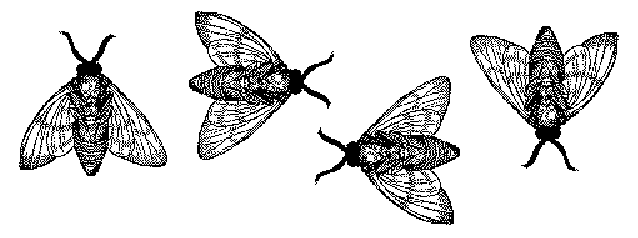
\includegraphics{flies}
%\caption{A sample black and white graphic
%that needs to span two columns of text.}
%\end{figure*}
%
%
%\begin{figure}
%\centering
%
\includegraphics[height=1in, width=1in]{rosette}
%\caption{A sample black and white graphic that has
%been resized with the \texttt{includegraphics} command.}
%\vskip -6pt
%\end{figure}
%
%\subsection{Theorem-like Constructs}
%Other common constructs that may occur in your article are
%the forms for logical constructs like theorems, axioms,
%corollaries and proofs.  There are
%two forms, one produced by the
%command \texttt{{\char'134}newtheorem} and the
%other by the command \texttt{{\char'134}newdef}; perhaps
%the clearest and easiest way to distinguish them is
%to compare the two in the output of this sample document:
%
%This uses the \textbf{theorem} environment, created by
%the\linebreak\texttt{{\char'134}newtheorem} command:
%%\newtheorem{theorem}{Theorem}
%\begin{theorem}
%Let $f$ be continuous on $[a,b]$.  If $G$ is
%an antiderivative for $f$ on $[a,b]$, then
%\begin{displaymath}\int^b_af(t)dt = G(b) - G(a).\end{displaymath}
%\end{theorem}
%
%The other uses the \textbf{definition} environment, created
%by the \texttt{{\char'134}newdef} command:
%\newdef{definition}{Definition}
%\begin{definition}
%If $z$ is irrational, then by $e^z$ we mean the
%unique number which has
%logarithm $z$: \begin{displaymath}{\log e^z = z}\end{displaymath}
%\end{definition}
%
%Two lists of constructs that use one of these
%forms is given in the
%\textit{Author's  Guidelines}.
% 
%There is one other similar construct environment, which is
%already set up
%for you; i.e. you must \textit{not} use
%a \texttt{{\char'134}newdef} command to
%create it: the \textbf{proof} environment.  Here
%is a example of its use:
%\begin{proof}
%Suppose on the contrary there exists a real number $L$ such that
%\begin{displaymath}
%\lim_{x\rightarrow\infty} \frac{f(x)}{g(x)} = L.
%\end{displaymath}
%Then
%\begin{displaymath}
%l=\lim_{x\rightarrow c} f(x)
%= \lim_{x\rightarrow c}
%\left[ g{x} \cdot \frac{f(x)}{g(x)} \right ]
%= \lim_{x\rightarrow c} g(x) \cdot \lim_{x\rightarrow c}
%\frac{f(x)}{g(x)} = 0\cdot L = 0,
%\end{displaymath}
%which contradicts our assumption that $l\neq 0$.
%\end{proof}
%
%Complete rules about using these environments and using the
%two different creation commands are in the
%\textit{Author's Guide}; please consult it for more
%detailed instructions.  If you need to use another construct,
%not listed therein, which you want to have the same
%formatting as the Theorem
%or the Definition shown above,
%use the \texttt{{\char'134}newtheorem} or the
%\texttt{{\char'134}newdef} command,
%respectively, to create it.
%
%\subsection*{A {\secit Caveat} for the \TeX\ Expert}
%Because you have just been given permission to
%use the \texttt{{\char'134}newdef} command to create a
%new form, you might think you can
%use \TeX's \texttt{{\char'134}def} to create a
%new command: \textit{Please refrain from doing this!}
%Remember that your \LaTeX\ source code is primarily intended
%to create camera-ready copy, but may be converted
%to other forms -- e.g. HTML. If you inadvertently omit
%some or all of the \texttt{{\char'134}def}s recompilation will
%be, to say the least, problematic.
%
%\section{Conclusions}
%This paragraph will end the body of this sample document.
%Remember that you might still have Acknowledgments or
%Appendices; brief samples of these
%follow.  There is still the Bibliography to deal with; and
%we will make a disclaimer about that here: with the exception
%of the reference to the \LaTeX\ book, the citations in
%this paper are to articles which have nothing to
%do with the present subject and are used as
%examples only.
%%\end{document}  % This is where a 'short' article might terminate
%
%%ACKNOWLEDGMENTS are optional
%\section{Acknowledgments}
%This section is optional; it is a location for you
%to acknowledge grants, funding, editing assistance and
%what have you.  In the present case, for example, the
%authors would like to thank Gerald Murray of ACM for
%his help in codifying this \textit{Author's Guide}
%and the \textbf{.cls} and \textbf{.tex} files that it describes.
%HERE

%
% The following two commands are all you need in the
% initial runs of your .tex file to
% produce the bibliography for the citations in your paper.
\bibliographystyle{abbrv}
\bibliography{reference}  % sigproc.bib is the name of the Bibliography in this case
% You must have a proper ".bib" file
%  and remember to run:
% latex bibtex latex latex
% to resolve all references
%
% ACM needs 'a single self-contained file'!
%
%APPENDICES are optional
%\balancecolumns

%HERE
%\appendix
%%Appendix A
%\section{Headings in Appendices}
%The rules about hierarchical headings discussed above for
%the body of the article are different in the appendices.
%In the \textbf{appendix} environment, the command
%\textbf{section} is used to
%indicate the start of each Appendix, with alphabetic order
%designation (i.e. the first is A, the second B, etc.) and
%a title (if you include one).  So, if you need
%hierarchical structure
%\textit{within} an Appendix, start with \textbf{subsection} as the
%highest level. Here is an outline of the body of this
%document in Appendix-appropriate form:
%\subsection{Introduction}
%\subsection{The Body of the Paper}
%\subsubsection{Type Changes and  Special Characters}
%\subsubsection{Math Equations}
%\paragraph{Inline (In-text) Equations}
%\paragraph{Display Equations}
%\subsubsection{Citations}
%\subsubsection{Tables}
%\subsubsection{Figures}
%\subsubsection{Theorem-like Constructs}
%\subsubsection*{A Caveat for the \TeX\ Expert}
%\subsection{Conclusions}
%\subsection{Acknowledgments}
%\subsection{Additional Authors}
%This section is inserted by \LaTeX; you do not insert it.
%You just add the names and information in the
%\texttt{{\char'134}additionalauthors} command at the start
%of the document.
%\subsection{References}
%Generated by bibtex from your ~.bib file.  Run latex,
%then bibtex, then latex twice (to resolve references)
%to create the ~.bbl file.  Insert that ~.bbl file into
%the .tex source file and comment out
%the command \texttt{{\char'134}thebibliography}.
%% This next section command marks the start of
%% Appendix B, and does not continue the present hierarchy
%\section{More Help for the Hardy}
%The sig-alternate.cls file itself is chock-full of succinct
%and helpful comments.  If you consider yourself a moderately
%experienced to expert user of \LaTeX, you may find reading
%it useful but please remember not to change it.
%%\balancecolumns % GM June 2007
%% That's all folks!
%HERE
\end{document}
